\documentclass[12pt, a4paper]{article}
\usepackage{iem} %enthaelt viele nuetzliche usepackages und definiert
\usepackage{listings} %source code listings
\lstset{
        language=Matlab,
        numbers=left,
        breaklines=true
}

% ein paar Reformatierungen
\hyphenation{}

\begin{document}
\selectlanguage{ngerman}

\title{Untersuchung verschiedener Upmixingmethoden für DirAC}

\author{Manuel Planton, BSc \\ Michael Hirschmugl, BSc\\\\\small{Betreuung: Dr. Franz Zotter, Dr. Matthias Frank}}

\markboth{}{M. Planton, M. Hirschmugl: DirAC Upmixing}

\doctype{Seminararbeit aus Algorithmen in Akustik und Computermusik 2}

\date{WS 2019/2020}

\maketitle
\newpage
\pagestyle{empty}
\hspace{1cm}\vspace{3cm}

\hspace{1cm}\vspace{1cm}

\begin{abstract}
   Diese Seminararbeit behandelt verschiedene Ausführungen und auch Optimierungen des DirAC-Verfahrens (Directional Audio Coding). Mit diesem Verfahren können Ambisonics Aufnahmen erster Ordnung in ihrer räumlichen Darstellung verbessert und auf eine höhere Ordnung hochgerechnet werden.
   Da die Aufnahme in Ambisonics erster Ordnung mit Hilfe von Soundfield Mikrofonen sehr einfach und günstig durchgeführt werden kann, jedoch eine wenig überzeugende Darstellung von Räumlichkeit und Klang bietet, kann ein solches Upmixing die Wiedergabe in vielerlei Hinsicht verbessern.
   Zu diesem Zweck sollen verschiedene DirAC-Implementierungen untereinander, und auch mit kommerziellen Plugins verglichen werden. Somit wird in dieser Seminararbeit die optimale Realisierung mit dem größten klanglichen Vorteil gesucht.
\end{abstract}
\selectlanguage{english}
\begin{abstract}
   This seminar project examines various designs and optimizations of DirAC (Directional Audio Coding), which is used for upmixing of first-order ambisonics recordings, in order to enhance spatial resolution.
   While soundfield microphones represent a straightforward method for the creation of first-order ambisonics recordings on a budget, the spatial representation is rarely convincing, and upmixing to higher order ambisonics is the prevalent procedure for the correction of such deficiencies.
   Hence, the goal of this project is to seek out the prime implementation of DirAC and to compare it to other upmixing approaches, as well as to different implementations of the DirAC algorithm itself.
\end{abstract}
\selectlanguage{ngerman}
\newpage
\pagestyle{myheadings}
\hspace{1cm}\vspace{2cm}

\tableofcontents
\newpage

\section{Einleitung}
Räumliche Klangfeldaufzeichnungen in Ambisonics 1. Ordnung sind grundsätzlich vergleichsweise einfach und günstig zu realisieren. Mit der ambisonischen Ordnung steigen jedoch auch unterschiedliche Qualitätsmerkmale der einhüllenden Wiedergabe. Dazu zählen die Sweet-Area (der günstige Abhörbereich), die Klangqualität, sowie die räumliche Auflösung der Schallrichtungen \cite{ambi-book}. Es existieren bereits einige Verfahren in Theorie und Praxis, um Ambisonics 1. Ordnung in eine höhere Ordnung zu rechnen. Prinzipiell werden solche Verfahren unter dem englischen Begriff ``Upmixing'' zusammengefasst.

V. Pulkki hat mit DirAC (Directional Audio Coding) \cite{pulkki} einen Algorithmus vorgeschlagen, der zuallererst die Trennung von gerichteten und diffusen Schallanteilen in B-Format Signalen zum Ziel hat. Weiters können gerichtete Schallereignisse anschließend auf eine beliebige Lautsprecheranordnung dekodiert werden \cite{spatial-book}, und somit ist auch Upmixing möglich.

Das kommerzielle Plugin HARPEX von S. Berge und N. Barrett stellt eine weitere Möglichkeit dar. Die Funktionsweise beruht hier auf der Kombination von parametrischen und linearen Dekodierungsverfahren \cite{harpy2} und basiert stark auf einem Transkodierungsverfahren von 1. Ordnung Ambisonics zu binauralen Signalen \cite{harpy}. Ein ähnlichen Ansatz verfolgen die COMPASS-Plugins von L. McCormack und A. Politis \cite{compy}, welche wiederum frei verfügbar sind.

Für Upmixing stehen daher theoretisch einige Methoden zur Verfügung, welche allerdings ausschlaggebende Qualitätsunterschiede an den Tag legen. Speziell DirAC unterscheidet sich bereits in den Realisierungsvarianten sehr stark, was die Synthese des dekorrelierten Diffusfeldes betrifft. Auch ist bisher unklar, ob die Dekodierung in ambisonisches B-Format höherer Ordnung grundsätzlich differenzierbar zur direkten Dekodierung auf die wiedergebende Lautsprecheranordnung bewertet wird.

In dieser Seminararbeit werden verschiedene Implementierungen des DirAC-Algorithmus und die erwähnten Plugins untereinander verglichen. Hierzu wird im Abschnitt 2 die Theorie zu DirAC erläutert. Ausgehend von einer psychoakustischen Annahme wird die allgemeine Funktionsweise des Algorithmus, sowie die spezielle Funktionsweise der DirAC-Implementierungen für diesen Versuch erklärt. Der Abschnitt schließt mit einem Überblick der verwendeten Dekorrelationsverfahren.

Die Evaluierung erfolgt in einem Hörversuch. Abschnitt 3 beschäftigt sich mit den Zielen, dem Aufbau und mit dem Konzept dieses Hörversuchs, dessen Ergebnisse schließlich präsentiert und diskutiert werden.

\section{DirAC}
In diesem Kapitel wird die prinzipielle Funktionsweise von DirAC (Directional Audio Coding) erläutert sowie die Implementierung in diesem Projekt beschrieben. Im Hörversuch wurden jedoch unterschiedliche Implementierungen des DirAC-Verfahrens untersucht, wobei sich diese einerseits durch die gewählte Methode der Diffusitätssynthese, und weiters auch durch zwei verschiedene Dekodierungsansätze unterscheiden. Die untersuchten Methoden zur Synthese von diffusen Audiosignalen umfassen neben einem Random-Phase-Algorithmus, welcher direkt in Octave ausprogrammiert wurde, auch bereits erhältliche Plugins wie ein Widening und ein FDN-Plugin aus der IEM Plugin Suite. Die beiden Ansätze zur Dekodierung von Ambisonics auf Lautsprechersignale bestehen einerseits aus einer direkten Dekodierung auf die abgezielte Lautsprecheranordnung, und weiters die Dekodierung auf eine T-Design Lautersprecheranordnung, welche eine größere Flexibilität bei der Wiedergabe bieten soll.

DirAC ist ein Algorithmus von Ville Pulkki \cite{pulkki} zum Upmixing für Koinzidenzmikrofon-Anordnungen wie FOA (First Order Ambisonics). Das Ziel des Algorithmus ist eine Erhöhung der Lokalisationsschärfe bei gleichzeitiger Verbesserung der Qualität der räumlichen Wiedergabe.
    \subsection{Annahmen aus der Psychoakustik} \label{annahmen}
    Die Funktionsweise des DirAC Algorithmus basiert nach Pulkki \cite{pulkki} auf 4 psychoakustischen Annahmen, aus denen sich eine resultierenden Annahme formulieren lässt.

\begin{enumerate}
    \item Die wahrgenommene Schalleinfallsrichtung (DOA: direction of arrival) wird bestimmt von der interauralen Zeitdifferenz (ITD: interaural time difference), von der interauralen Pegeldifferenz (ILD: interaural level difference) und von monauralen cues.
    \item Die wahrgenommene \textit{Diffusität} des Schalls wird von der interauralen Kohärenz bestimmt.
    \item Die wahrgenommene Klangfarbe des Schalls hängt vom Spektrum, der ITD, der ILD und von der interauralen Kohärenz ab.
    \item Die wahrgenomme Richtung wird bestimmt von der DOA, der Diffusität und vom Spektrum des Schalls, gemessen in einer Richtung mit Zeit-/Frequenzauflösung des menschlichen Ohrs.
\end{enumerate}

Die resultierende Annahme aus diesen 4 Annahmen ist, dass Menschen zu einem Zeitpunkt nur einen cue pro kritischer Bandbreite dekodieren können.

    \subsection{Funktionsweise}
    text

        \paragraph{Allgemein}
        In Abbildung \ref{fig:dirac_flow_general} ist das Prinzip des DirAC Algorithmus zu sehen. Die $M$ Mikrofonkanäle werden mittels STFT (oder Filterbank) in den Frequenzbereich gebracht. Es wird ein Pseudointensitätsvektor gebildet (ähnlich dem $r_e$-Vektormodell aus \cite{ambi-book}), der im Analyseschritt verwendet wird, um die Diffusität $\Psi$ und Schalleinfallsrichtung $D$ pro Frequenzband des Signals zu ermitteln. Hier fließt die resultierende psychoakustische Annahme ein (siehe \ref{annahmen}), weswegen nur eine Richtung pro Frequenzband ermittelt wird.

\begin{figure}[!ht]
  \centering
  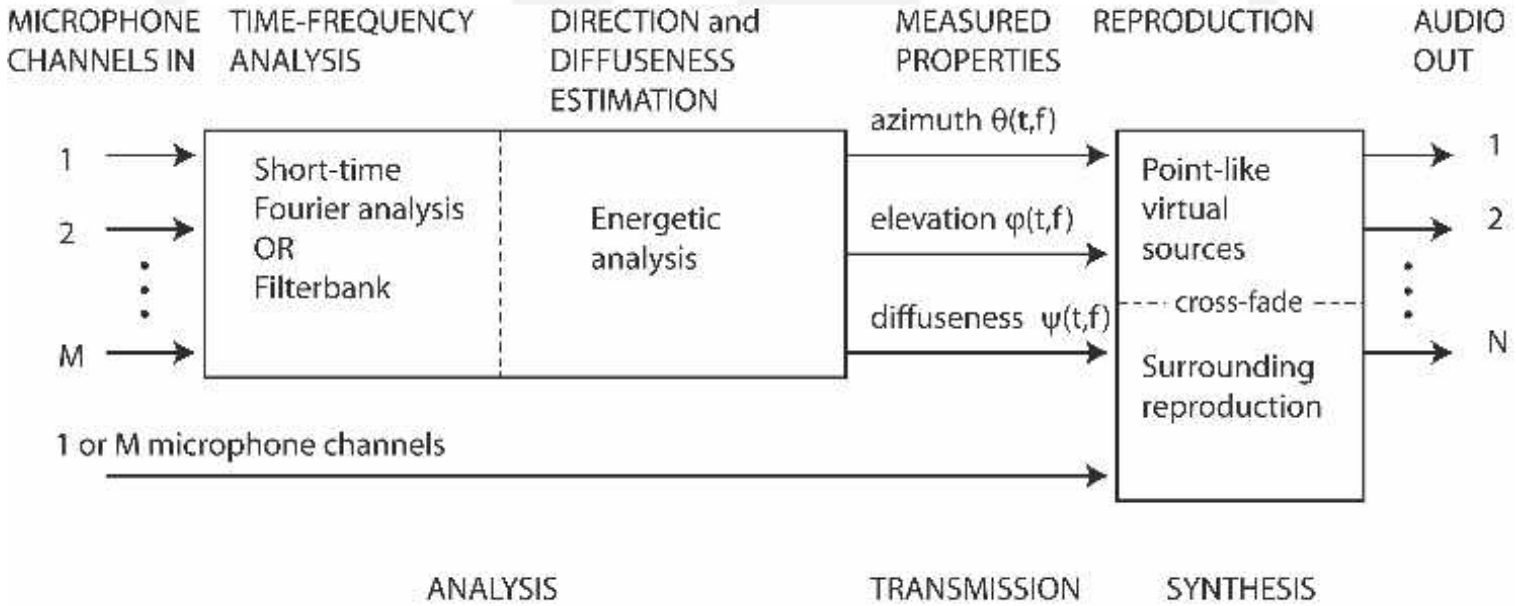
\includegraphics[width=0.9\textwidth]{funktionsweise/pic/pulkki_dirac_flow.png}
  \caption{Prinzip des DirAC Algorithmus\protect\footnotemark}
  \label{fig:dirac_flow_general}
\end{figure}

\footnotetext{Quelle: \cite{pulkki}}

Aus den $M$ Eingangskanälen werden mit virtuellen Mikrofonen die $N$ Ausgangskanäle gebildet (siehe Abbildung \ref{fig:dirac_flow_high}). Mit den ermittelten Eigenschaften werden die $N$ Kanäle spektral in einen gerichteten Anteil und in einen Diffusanteil getrennt. Der gerichtete Anteil hat bereits eine höhere Auflösung als die Eingangskanäle. Der Diffusanteil wird mit einem Dekorrelationsverfahren zur Erhöhung der Diffusität bearbeitet (siehe \ref{dekorrelation}). Anschließend werden die beiden Signalanteile per Addition wieder zusammengebracht und via iSTFT wieder in den Zeitbereich transformiert.

\begin{figure}[!ht]
  \centering
  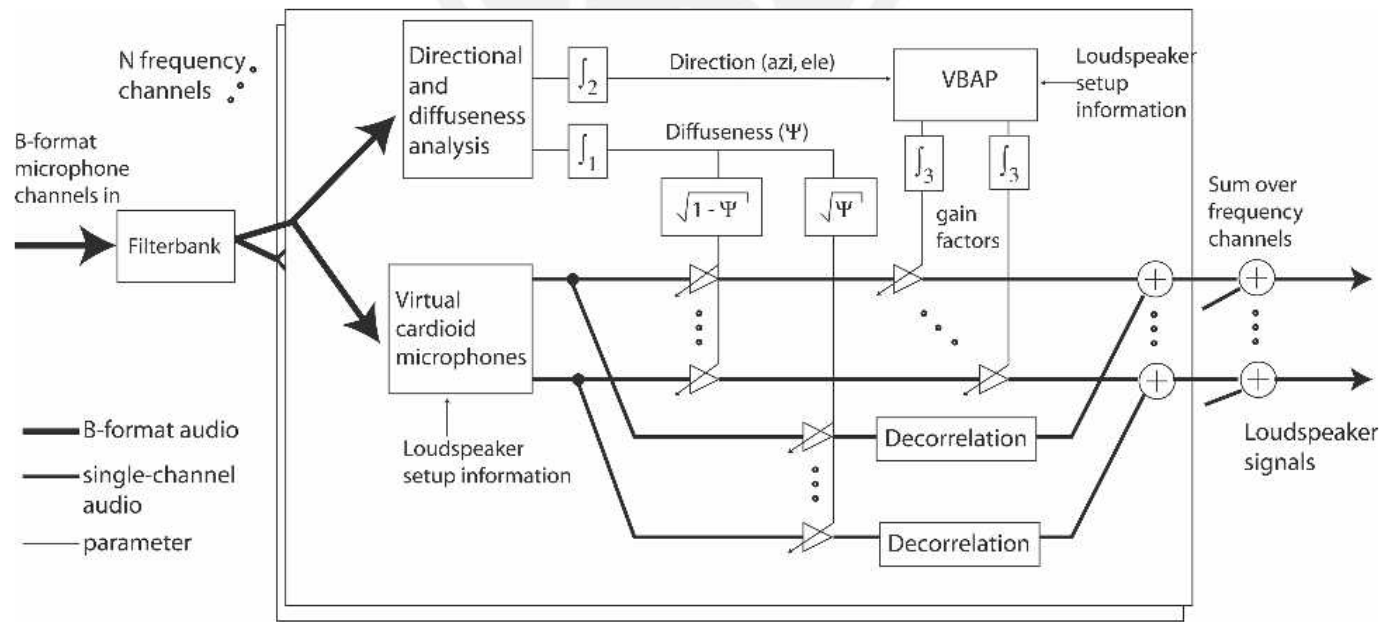
\includegraphics[width=0.9\textwidth]{funktionsweise/pic/pulkki_dirac_flow_2.png}
  \caption{DirAC zur hochqualitativen Reproduktion von B-Format Signalen\protect\footnotemark}
  \label{fig:dirac_flow_high}
\end{figure}

\footnotetext{Quelle: \cite{pulkki}}

In dieser Seminararbeit (und dem Hörversuch) wird ausschließlich diese Variante des DirAC-Algorithmus verwendet, der für eine hohe Audioqualität entwickelt wurde. In Abbildung \ref{fig:dirac_flow_low} ist eine andere Variante abgebildet, bei der die Signalübertragung eine größere Rolle spielt. Die Integralzeichen in den Abbildungen symbolisieren eine zeitliche Mittelung der Parameter zur Vermeidung von Artefakten.

\begin{figure}[!ht]
  \centering
  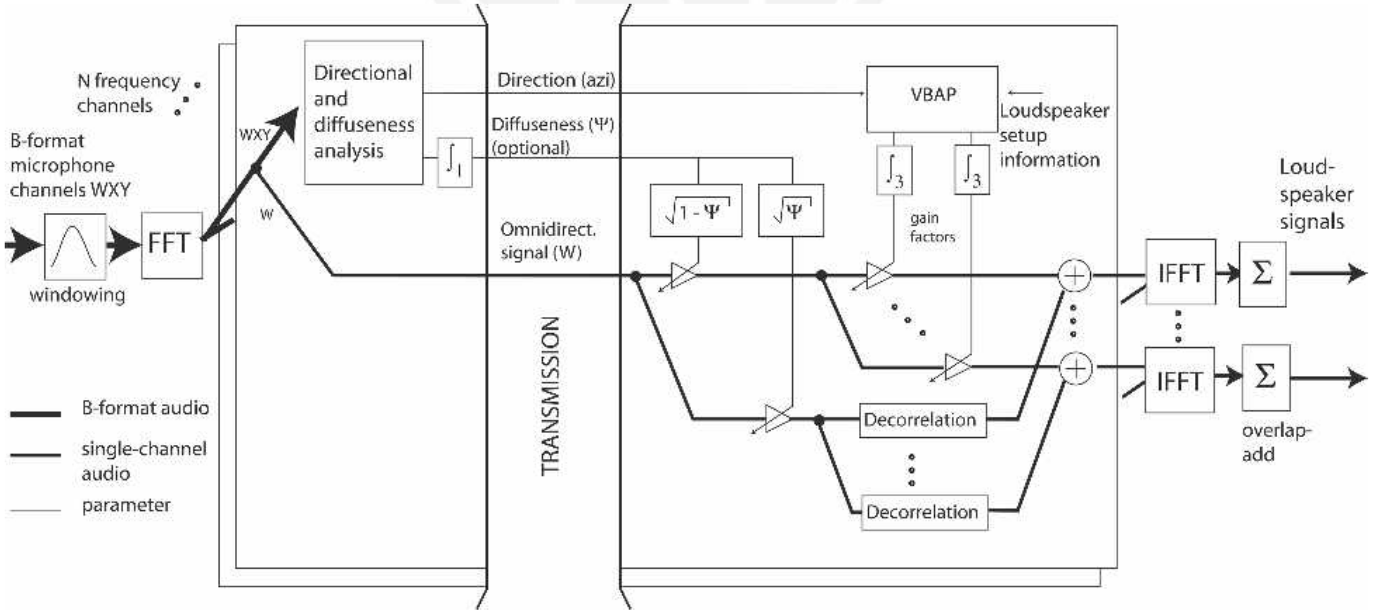
\includegraphics[width=0.9\textwidth]{funktionsweise/pic/pulkki_dirac_flow_3.png}
  \caption{DirAC für Telekommunikation\protect\footnotemark}
  \label{fig:dirac_flow_low}
\end{figure}

\footnotetext{Quelle: \cite{pulkki}}

    \subsection{Implementierung}
    In diesem Abschnitt wird beschrieben, wie der DirAC-Algorithmus in diesem Projekt implementiert wurde. Die Implementierung liegt als Script für GNU Octave vor und nutzt das \textit{signal}-Package. Der Code dafür ist zu großen Teilen direkt dem Buch \textit{Parametric Time-Frequency Domain Spatial Audio} ~\cite{spatial-book} von V. Pulkki entnommen.

\paragraph{Übersicht}
Zu Beginn des Skriptes wird das Eingangssignal im B-Format erster Ordnung eingelesen. Dieses muss als \textit{.wav}-Datei vorliegen und genau vier Kanäle (in der Reihenfolge $w$, $x$, $y$, $z$) umfassen. Die Samplerate wird direkt aus dieser Datei ermittelt und als Variable \textit{fs} im Workspace von GNU Octave gespeichert.

Anschließend wird eine Liste von Lautsprecherpositionen eingelesen. Dabei handelt es sich entweder um die Anordnung des einhüllenden Wiedergabesystems (z.B. 12 Lautsprecher im Produktionsstudio des IEM Graz), oder eine allgemeine t-Design Anordnung (in diesem Fall 48 Punkte für ein 9-Design). Die Koordinaten werden in sphärische Richtungen umgerechnet und daraus eine dreidimensionale VBAP-Matrix berechnet. Die Anzahl der Spalten dieser Matrix entspricht der Anzahl der eingelesenen Positionen (12 oder 48). Die Zeilenanzahl ist abhängig von der gewählten Richtungsauflösung (= 1 Grad). Diese Matrix dient dazu, gerichtete Audiosignale auf die Ausgabekanäle (reale Lautsprecheranordnung oder allgemeines t-Design) abzubilden.

Im nächsten Schritt wird eine Dekodierungsmatrix von virtuellen Mikrofonen erzeugt, um die vier Eingangskanäle $w[n]$, $x[n]$, $y[n]$ und $z[n]$ des B-Format-Signals auf die Ausgangskanäle (12 oder 48) dekodieren zu können. Dabei wird eine Supernieren-Charakteristik eingesetzt.

Das B-Format Eingangssginal wird anschließend in einer Schleife in zeitlichen Blöcken (Fenster) verarbeitet. Ein Fenster besteht dabei aus jeweils 512 Samples und wird in einer 1024-Punkt Fouriertransformation mit der Hilfe der Funktion \textit{fft()} in den Frequenzbereich transformiert. Die FFT-Länge wurde als doppelte Blocklänge gewählt um Aliasing zu vermeiden. Die zeitlichen Blöcke werden noch mit einem Hann-Fenster für die Resynthese beaufschlagt. Ein Hann-Fenster kann in Octave mit der Funktion \textit{hann()} (alternativ: \textit{hanning(), abgeleitet von ``to hann''}) erzeugt, und einfach als Vektor mit den Zeitsignalen multipliziert werden.
        \paragraph{Analyse von Richtungs- und Diffusanteil}
        Zur Bestimmung von Richtungs- und Diffusanteil werden zunächst Schallschnelle und Energie berechnet. Die Schnallschnelle wird als Vektor $\textbf{V}_{m}[k] = [X_{m}[k], Y_{m}[k], Z_{m}[k]]$ aus den gerichteten Anteilen (der Druckgradienten-Mikrofone) des B-Format Signals bestimmt. Der Schalldruck ist der omnidirektionale Anteil $W_{m}[k]$. Die Indizes $m$ und $k$ werden hier zur Kennzeichnung des Zeitfensters als Funktion der Frequenzzahl $k$ verwendet.

Der Pseudo-Schallintensitätsvektor $\textbf{I}_{m}[k]$ wird aus dem Schnellevektor und dem konjugiert komplexen Schalldruck in Gleichung \ref{eq:inten} abgeleitet, wobei hier rein der Realteil heranzogen wird, da sonst die Blindeinteile des Schnellevektors das Ergebnis verfälschen würden \cite{pulkki}. Der Intensitätsvektor stellt bereits die Schalleinfallsrichtung für alle Frequenzbins einzeln dar, jedoch entgegengesetzt der Einfallsrichtung $\textbf{D}_{m}[k]$

\begin{equation}
    -\textbf{D}_{m}[k] = \textbf{I}_{m}[k] = \Re(W_{m}[k]^{*} \cdot \textbf{V}_{m}[k]) .
    \label{eq:inten}
\end{equation}

Die Schallenergie $E_{m}[k]$ wird mit Hilfe der Gleichung

\begin{equation}
    E_{m}[k] = \frac{|W_{m}[k]|^2+||\textbf{V}_{m}[k]||^2}{2}
    \label{eq:energy}
\end{equation}

ausgewertet.

Um Sprünge in der Lautsprecherzuordnung von gerichteten Signalen bei raschen Bewegungen zu vermeiden, wird der Intensitätsvektor zusätzlich durch eine zeitliche Mittelwertbildung geglättet. Diese Glättung kann im Skript mit einer frequenzabhängigen Zeitkonstante vorgegeben werde. Zusätzlich wird auch der Energievektor zeitlich geglättet. Anschließend wird der Intensitätsvektor verwendet, um die Einfallsrichtungen in sphärischen Koordinaten zu bestimmen.

Die Diffusität $\psi_{m}[k]$ kann schlussendlich aus dem Vergleich des Betrags des Intensitätsvektors mit der Energie ermittelt werden

\begin{equation}
    \psi_{m}[k] = \sqrt{1 - \frac{||\mathbb{E}(\textbf{I}_{m}[k])||}{\mathbb{E}(E_{m}[k])}} .
    \label{eq:diff}
\end{equation}

 Der Erwartungswert entspricht hier den (zeitlich) gemittelten Vektoren.

%\begin{figure}[!ht]
%  \centering
%  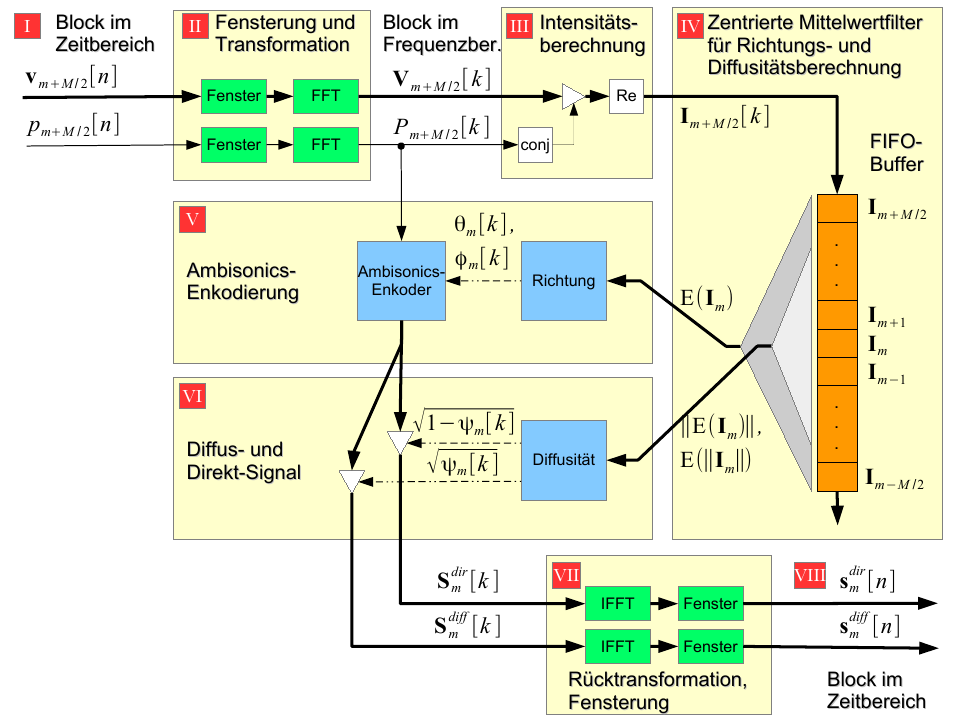
\includegraphics[width=0.7\textwidth]{implementierung/plots/flow.png}
%  \label{fig:flow}
%  \caption{Flussdiagram des DirAC Algorithmus in Octave \cite{seminar2016}}
%\end{figure}
        \paragraph{Upmixing auf Lautsprecherandordnung}
        

%Zur Dekodierung auf eine bestimmte Lautsprecheranordnung wird eine Matrix aus virtuellen Mikrofonen berechnet, woraus sich eine Tabelle mit Gain-Werten ergibt. Diese Tabelle besteht aus einer Spalte für jeden Lautsprecherkanal und kann die einzelnen Frequenzbins in einem VBAP-Verfahren den enstprechenden Lautsprechern zuordnen. In dieser Seminararbeit wurden dabei zwei Ansätze für die Dekodierung verglichen: Einerseits die direkte Dekodierung auf die physische Lautsprecheranordnung des Wiedergabesystems, und andererseits ein allgemeiner Ansatz womit die Dekodierung auf eine t-Design Lautsprecheranordnung erfolgt. Dieser Dekodierungsansatz hat den Vorteil, dass die Wiedergabeanordnung zum Zeitpunkt des Upmixings nicht vorgegeben sein muss. Auch für die Klangqualität ergeben sich daraus Vorteile, welche im Hörversuch besprochen werden.

Im Frequenzbereich wird jeder Spektralblock mit dem Sampling-Dekoder dekodiert, um die vier Eingangskanäle in eine höhere Kanalzahl zu wandeln.
In dieser Seminararbeit wurden dabei zwei Ansätze für die Dekodierung verglichen: Einerseits die direkte Dekodierung auf die physische Lautsprecheranordnung des Wiedergabesystems, und andererseits ein allgemeiner Ansatz womit die Dekodierung auf ein t-Design erfolgt. Dieser Dekodierungsansatz hat den Vorteil, dass die physische Lautsprecheranordnung zum Zeitpunkt des Upmixings nicht gegeben sein muss.

Bei einem 9-Design (Abb. \ref{fig:tdesign_image}) ergibt sich eine sphärische Anordnung von 48 virtuellen Lautsprechern, welche eine optimale dekodierung des B-Formats erlaubt.

\begin{figure}[!ht]
  \centering
  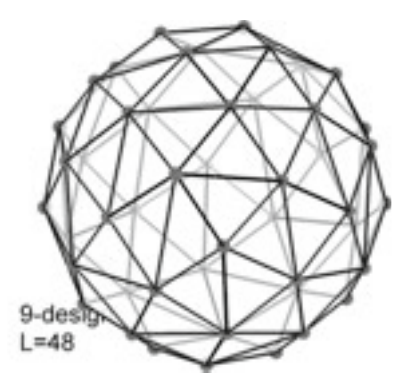
\includegraphics[width=0.35\textwidth]{implementierung/plots/t-design.png}
  \caption{9-Design T-Design \cite{ambi-book}}
  \label{fig:tdesign_image}
\end{figure}

%Zur Dekodierung wird in Octave also eine Matrix mit Lautsprechergewichten für Schalleinfallsrichtungen erstellt. Somit kann einer gegebenen frequenzabhängigen Richtung (bestehend aus Azimuth und Elevation), ein bestimmter Gain-Wert am entsprechenden Lautsprecherkanal zugeordnet werden.

        \paragraph{Trennung von Diffus- und Richtungsanteil}
        %Die Trennung von Diffus- und Richtungsanteil erfolgt im Frequenzbereich, wobei beide Anteile aus dem omindirektionalen Anteil des B-Format Signals durch gewichtete Filterung erzeugt werden. Prinzipiell wird für den gerichteten Anteil ein spektraler Block im Frequenzbereich mit zwei Matrizen multipliziert: Einerseits mit der VBAP-Tabelle um die Richtung einem Lautsprecher zuzuordnen, und andereseits mit dem ebenfalls frequenzabhängigen Diffusitätsvektor. Somit werden Frequenzbins mit frequenzabhängigen Diffusitätswerten gewichtetet, und diesen anschließend entsprechende Lautsprechergewichte zugeordnet.

%Nach der Berechnung des gerichteten Signalanteils kann auch der Diffusanteil aus dem omnidirektionalen Signal erzeugt werden. Dieser entspricht lediglich dem nicht-gerichteten Anteil des omnidirektionalen Signals und wird daher aus der Filterkurve des Direktanteils bestimmt. Somit ergeben sich an dieser Stelle zwei frequenzabhängige Signalmatrizen für Diffus- und Richtungsanteil. Beide Matrizen besitzen eine Spalte für jeden Lautsprecherkanal und die Zeilenzahl entspricht der FFT-Länge.

Die Trennung von Diffus- und Richtungsanteil erfolgt ebenfalls im Frequenzbereich. Der frequenzabhängige Diffusitätsvektor wird hier verwendet, um den gerichteten Anteil aus den dekodierten Signalen (mit 12 oder 48 Kanälen) zu filtern. Prinzipiell wird für den gerichteten Anteil ein spektraler Block mit zwei Matrizen multipliziert: Erstens mit dem frequenzabhängigen Diffusitätsvektor, und weiters mit der VBAP-Tabelle um die gerichteten Signale den entsprechenden Lautsprechern zuzuordnen. Somit werden Frequenzbins mit frequenzabhängigen Diffusitätswerten gewichtetet, und diesen anschließend entsprechende Lautsprechergewichte verliehen.

Nach der Berechnung des gerichteten Signalanteils kann auch der Diffusanteil aus den dekodierten Signalen erzeugt werden. Dieser entspricht dem nicht-gerichteten Anteil und wird daher aus der Filterkurve des Direktanteils bestimmt. Somit ergeben sich an dieser Stelle zwei frequenzabhängige Signalmatrizen für Diffus- und Richtungsanteil für jedes zeitliche Verarbeitungsfenster. Beide Matrizen besitzen eine Spalte für jeden Wiedergabekanal und die Zeilenzahl entspricht der FFT-Länge.
        \paragraph{Resynthese}
        Die Resynthese entspricht einem gewöhnlichem Overlap-Add Verfahren und erzeugt mittel inverser Fast Fourier Transformation wieder Zeitsignale aus den Matrizen für Richtungs- und Diffusanteil. An dieser Stelle kann optional weiters die Dekorrelation des Diffusanteils durchgeführt werden.


    \subsection{Dekorrelationsverfahren} \label{dekorrelation}
    Wie bereits in den psychoakustischen Annahmen beschrieben, ist die Diffusität des wahrgenommenen Schalls abhängig von der interauralen Dekorrelation der Ohrsignale. In einem vollkommen diffusen Schallfeld trifft der Schall aus allen Richtungen auf den Hörer, was stark dekorrelierte Ohrsignale zur Folge hat. Die Aufgabe des Dekorrelationsverfahrens in diesem Versuch, ist die Synthese der Diffussignale für die Lautsprecherwiedergabe. Das Dekorrelationsverfahren soll somit stark dekorrelierte Lautsprechersignale zur Verfügung stellen, um die Diffusität des erzeugten Schallfeldes zu gewährleisten, ohne Artefakte zu erzeugen.

Es wurden drei Dekorrelationsverfahren verglichen. \textit{Random Phase} ist die originale DirAC Methode und weiters wurde ein \textit{Feedback Delay Network} und \textit{Widening} verwendet, die beide als Plugin verfügbar waren.

\paragraph{Random Phase}
Bei diesem Verfahren wird das Diffussignal mit weißem Rauschen gefaltet. Dabei ändert sich das Betragsspektrum des Signals nicht, aber das Phasenspektrum wird zufällig. Damit die Lautsprechersignale dekorreliert sind, müssen sich die Rauschsignale für die Faltung unterscheiden. Um Artefakte zu vermeiden, werden in drei Frequenzbereichen exponentiell abfallende Rauschsignale mit unterschiedlichen Zeitkonstanten verwendet.

\paragraph{Feedback Delay Network}

In Abbildung ~\ref{fig:fdn} ist ein Feedback Delay Network (FDN) für drei Signale zu sehen. Die Eingangssignale werden mit Delays zeitverzögert, deren Länge $M_i$ Primzahlverhältnisse haben sollen, um ausgeprägte Resonanzen zu vermeiden.

Die verzögerten Eingangssignale werden anschließend über eine Mischungsmatrix (Glg. ~\ref{eq:mischmat}) zurückgeführt, um eine möglichst randomisierte Durchmischung zu erreichen.

\begin{equation}
    Q = 
    \begin{pmatrix}
		q_{11} & q_{12} & q_{13} \\
        q_{21} & q_{22} & q_{23} \\
        q_{31} & q_{32} & q_{33} \\
    \end{pmatrix}
    \label{eq:mischmat}
\end{equation}

Die gemischten Signale werden noch mit den Verstärkungsfaktoren $g_i$ multipliziert und schließlich zu den Eingangssignalen addiert. Das Verhalten des FDN hängt maßgeblich von den Delay-Längen $M_i$ und von den Eigenschaften der Mischungsmatrix $Q$ ab.

Prinzipiell eignet sich ein FDN gut zur Simulation von späten Reflexionen. In diesem Versuch wurden sehr kurze Nachhallzeiten verwendet, um die Diffusität der Signale zu erhöhen, ohne den Eindruck eines zusätzlichen Raums durch das FDN zu verursachen.

\begin{figure}[!ht]
  \centering
  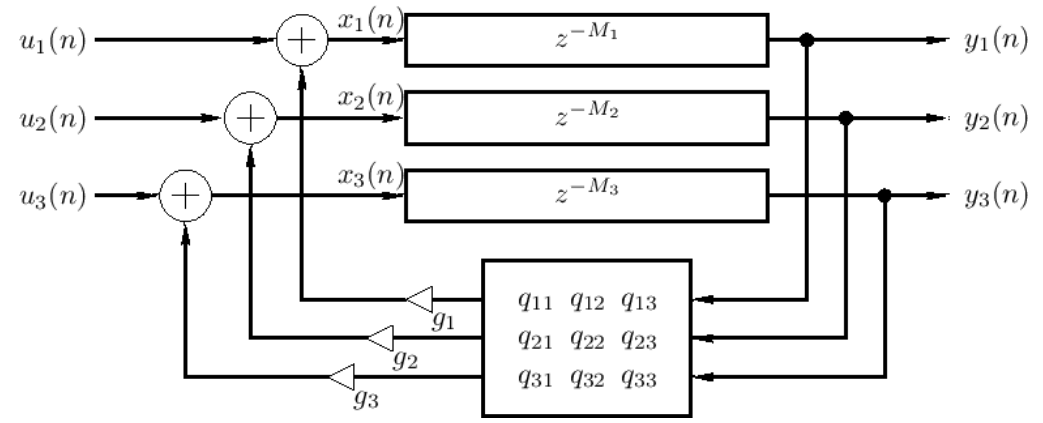
\includegraphics[width=0.9\textwidth]{dekorrelation/pic/FDN_smith.png}
  \caption{Feedback Delay Network für 3 Signale (Smith) \protect\footnotemark }
  \label{fig:fdn}
\end{figure}

\footnotetext{Quelle: \cite{fdn_smith}}

\paragraph{Widening}
Der Widening-Effekt wird durch frequenzabhängiges Panning um die Panning-Richtung erzeugt \cite{ambi-book}. Dabei werden aufeinanderfolgende Frequenzanteile in der Richtung leicht versetzt. Es kommt auch zu einer verschmierung der zeitlichen Feinstruktur des Signals. Dieser Effekt wird als Erhöhung der Distanz und Diffusität wahrgenommen und kann zur Simulation von frühen lateralen Reflexionen verwendet werden.



\section{Hörversuch}
Die unterschiedlichen Upmixing- und Dekorrelationsalgorithmen, sowie die beiden Dekodierungsmethoden, wurden anschließend in einem Hörversuch auf die Probe gestellt. Hierzu wurden verschiedene Ambisonics Aufnahmen im B-Format herangezogen und mit unterschiedlichen Kombinationen aus Upmixing, Diffusität und Dekodierung bearbeitet. Die Ergebnisse konnten dann direkt im Produktionsstudio des Instituts für elektronische Musik wiedergegeben und von Versuchspersonen bewertet werden. Der Augenmerk sollte dabei auf Klangqualität und Darstellung der Räumlichkeit liegen. Die folgenden Kapitel sollen die Annahmen, Hypothesen, den Aufbau und die Ergebnisse dieses Versuchs darstellen.

Generell kann der Hörversuch in die folgende vier Komponenten des Aufbaues und Versuchsdesigns zerlegt werden, welche anschließend im Kapitel \ref{aufbau_und_konzept} genauer erläutert werden:
\begin{itemize}
    \item Reaper Projekt gesteuert durch Mushra-Test
    \item Vergleich von 6 Algorithmen + Referenz
    \item Ausgehend von 4 verglichenen Testsignale
    \item Einschätzen von Klangqualität und Räumlichkeit
\end{itemize}

    \subsection{Ziele des Hörversuchs}
    Prinzipiell sollten mit dem Hörversuch folgende Forschungsfragen beantwortet werden:

\begin{itemize}
	\item Bietet das Upmixing durch DirAC auf ein ambisonisches Format höherer Ordnung einen Vorteil bezüglich der Darstellung von Räumlichkeit in der Aufnahme?
	\item Ist es möglich Upmixing mit DirAC ohne negative Beeinflussung der Klangqualität durchzuführen?
	\item Welche Kombination aus Dekorrelation und Dekodierung bietet dabei die (subjektiv) beste Wiedergabe der Klangqualität?
	\item Wie wird ein kommerzielles Plugin wie \textit{HARPEX} im Vergleich zu einer Lösung mit DirAC bewertet?
	\item Wie wird ein freies Plugin wie \textit{COMPASS} im Vergleich zu einer Lösung mit DirAC bewertet?
\end{itemize}

Weiters soll die Beschaffenheit des Ausgangssignals dabei einbezogen werden. Speziell geht es dabei um die Frage ob eine sehr diffuse Aufnahme ähnlich bewertet wird wie ein eher gerichtetes Signal im B-Format erster Ordnung.

In ersten Versuchen konnten wir die Algorithmen bereits selbst vergleichen und vermuteten daher, dass die Lokalisation und Darstellung der Räumlichkeit durch DirAC positiv beeinflusst werden kann, wenn dies auch durchaus von der eingesetzten Dekorrelationsmethode stark abhängig ist. Weiters wurde angenommen, dass eine bestimmte Kombination von Algorithmen durchaus vergleichbare Ergebnisse mit dem kommerziellen HARPEX-Plugin bieten könnte. Speziell die Dekodierung auf das 9-Design mit 48 virtuellen Schallquellen könnte Vorteile in der Wiedergabe bieten, da die geringen Abstände bei einer derartig dichten Anordnung virtueller Quellen zu weniger Richtungssprüngen führen.

    \subsection{Aufbau und Konzept}
    \label{aufbau_und_konzept}
    \paragraph{Ausgangssignale}
Es wurden insgesamt vier unterschiedliche Aufnahmen als Testsignale herangezogen. Davon wurden zwei Aufnahmen im B-Format synthetisch erzeugt, um auch sehr gerichtete Signale vergleichen zu können:

\begin{itemize}
	\item Synthetisches Zirpen mit Elevationswinkel $\vartheta=0^{\circ}$, rotierend in Azimuth mit Winkelgeschwindigkeit $\omega=90^{\circ}/s$
	\item Synthetisches Zirpen mit Elevationswinkel $\vartheta=0^{\circ}$, rotierend in Azimuth mit Winkelgeschwindigkeit $\omega=90^{\circ}/s$, nachträglich verhallt mittels FDN-Plugin
	\item Live-Musik Aufnahme mit Besetzung:
	\begin{itemize}
	  \item Schlagzeug
	  \item E-Bass
	  \item Cello
	  \item Piano
	\end{itemize}
	\item Umgebungsgeräusche Straßenkreuzung
\end{itemize}

Die synthetischen Signale wurden dabei mit Hilfe eines weiteren Skriptes in Octave produziert. Das zusätzlich verhallte Signal wurde in Reaper mit dem FDN Reverb Plugin aus der IEM Plugin Suite\footnote{IEM Plugin Suite: \url{https://plugins.iem.at/}} nachträglich bearbeitet. Dies soll einen direkteren Vergleich der Performance von stark gerichtetem und stark diffusem Signal bieten. Die Live-Musik Aufnahme wurde im IEM Cube angefertigt und bietet einen ausgeprägten räumlichen Eindruck, wobei die Ambience-Aufnahme an einer Straßenkreuzung die größte Diffusität aufweist. Diese Aufnahmen wurden mit Soundfield Mikrofonen durchgeführt. Somit werden im Hörversuch vier sehr unterschiedliche Aufnahmeszenarien verwendet.


\paragraph{Verglichene Kombinationen von Dekorrelation und Dekodierung}

Die folgende Liste zeigt die verglichenen Kombinationen aus Upmixing-, Dekorrelations- und Dekodierungsmethoden:

\begin{itemize}
	\item LSDecorr: DirAC, 12 Lautsprecher + Random Phase Decorrelation
	\item LSFDN: DirAC, 12 Lautsprecher + FDN Decorrelation
	\item TdesFDN: DirAC, t-Design + FDN Decorrelation
	\item TdesWid: DirAC, t-Design + Widening Plugin
	\item HARPEX\footnote{HARPEX: \url{https://harpex.net/index.html}}
	\item COMPASS\footnote{COMPASS: \url{http://research.spa.aalto.fi/projects/compass_vsts/plugins.html}}
\end{itemize}




Abbildung ~\ref{fig:algos} ist eine schematische Darstellung der Wiedergabe der Testsignale. Die Wiedergabe ist grundsätzlich immer eine Kombination aus vorhergehender Erzeugung und Bearbeitung in einem Octave-Skript, und Wiedergabe und Bearbeitung in Reaper mittels Plugins.

\begin{figure}[!ht]
  \centering
  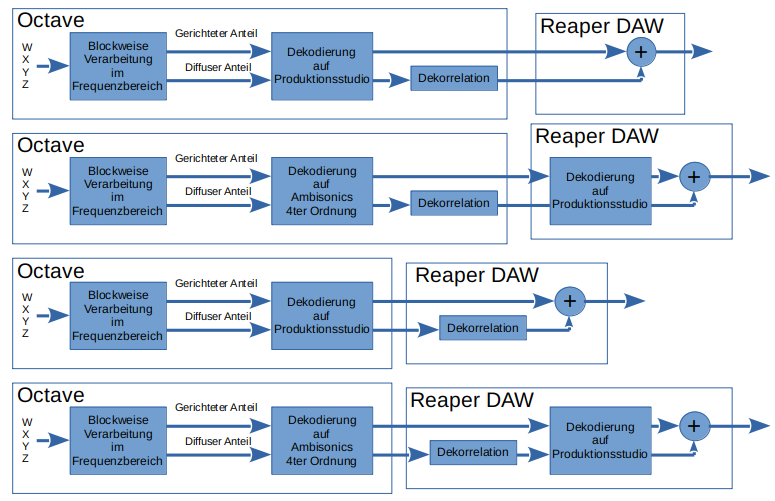
\includegraphics[width=1\textwidth]{aufbau/plots/algos.png}
  \label{fig:algos}
  \caption{Flussdiagram Wiedergabe im Produktionsstudio}
\end{figure}

Die Dekodierung der ambisonischen Signale wird für alle Signale in GNU Octave durchgeführt. Nach dem DirAC-Upmixing wird die Dekodierung entweder auf die 12-Lautsprecher-Anordnung des Produktionsstudios, oder allgemein für ein 9-Design ausgeführt. Daher können die 12-Lautsprecher-dekodierten Signale in Reaper anschließend direkt auf die Lautsprecher ausgerichtet wiedergegeben werden, und das t-Design-Signal wird zuvor noch mit einem Dekodierungsplugin auf die Lautsprecher aufgeteilt.

\paragraph{Wiedergabesystem}
Als Wiedergabesytem wurde die Lautsprecheranordnung des Produktionsstudios des IEM verwendet. Prinzipiell besteht die Lautsprecheranordnung im Produktionsstudio aus zwei übereinander liegenden horizontalen Ringen und einem Zenit-Lautsprecher. Es werden insgesamt 12 Lautsprecher verwendet, jedoch befinden sich keine Lautsprecher in vertikaler Richtung unter dem Horizont. Eine Visualisierung der Lautsprecheranordnung ist in Abb. ~\ref{fig:aufb:prodstud} dargestellt. Der Nadir-Lautsprecher in der Abbildung ist ein imaginärer Lautsprecher um Signale unter dem Horizont auf andere Lautsprecher zu verteilen.

\begin{figure}[!ht]
  \centering
  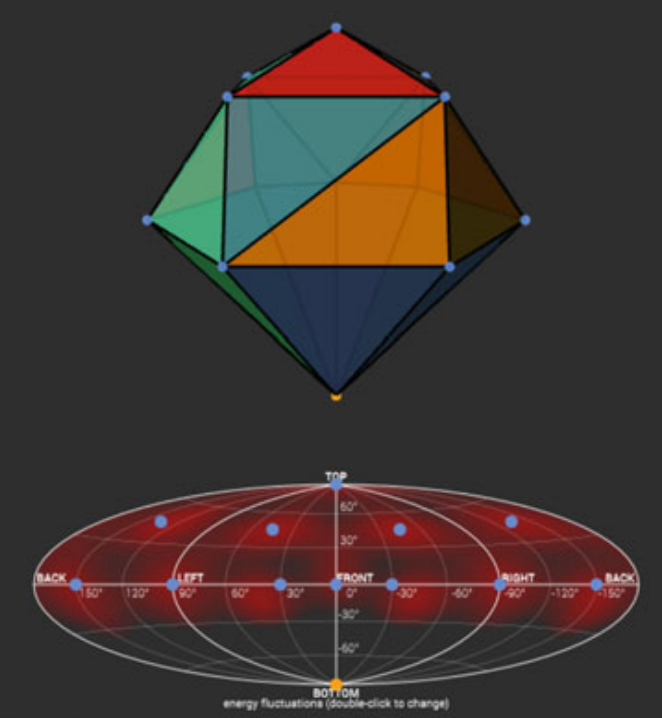
\includegraphics[width=0.4\textwidth]{aufbau/plots/speaker_pos_prod_studio.png}
  \caption{Visualisierung der Lautsprecheranordnung im Produktionsstudio des IEM \protect\footnotemark}
  \label{fig:aufb:prodstud}
\end{figure}

\footnotetext{Quelle: \cite{ambi-book}}

Im Falle unseres Hörversuchs muss unbedingt angemerkt werden, dass der Center-Lautsprecher im horizontalen Ring fehlte. Dies führt natürlich zu einer schlechteren Lokalisierbarkeit und höheren Quellbreite an dieser Stelle. Da dieses Verhalten bei allen Algorithmen und für alle Versuchspersonen gleich war, wurde der Hörversuch jedoch trotzdem durchgeführt.

\paragraph{Versuchsinterface}
Um die Antworten der Versuchspersonen auszuwerten wurde eine Anwendung eingesetzt, die einen MUSHRA-Test realisiert (MUltiple Stimuli with Hidden Reference and Anchor). Diese Anwendung wird über eine \textit{.json}-Datei konfiguriert und kann als Steuerung für die Reaper DAW verwendet werden. Die Anwendung teilt die Zeitspur der DAW in \textit{scenes} auf. Unterschiedliche Klangbeispiele werden daher als Marker zeitlich geordnet. Die verglichenen Algorithmen werden als Spuren in der DAW gesteuert. Schaltet man einen Algorithmus ein, um ihn hörbar zu machen, wird also ein Regler einer Spur in Reaper auf 0dB aufgezogen. Die FOA-Referenz wurde in den getesteten Algorithmen ebenfalls inkludiert.

Die MUSHRA-Anwendung stellt alle Algorithmen in randomisierter Reihenfolge auf einer eigenen Seite für jede Szene (Klangbeispiel) dar. Dadurch kann die Versuchsperson bei einem Hörbeispiel alle möglichen Algorithmen vergleichen und mit Schiebereglern auf einer quasi-kontinuierlichen Skala bewerten. Wenn eine Szene bewertet wurde kann die Versuchsperson zur nächsten wechseln.

    \subsection{Ergebnis}
    Das Ergebnis des Hörversuchs ist in Abbildung ~\ref{fig:versuch} zu sehen. Es wurden insgesamt 6 Personen mit geschultem Gehör befragt.

\begin{figure}[!ht]
  \centering
  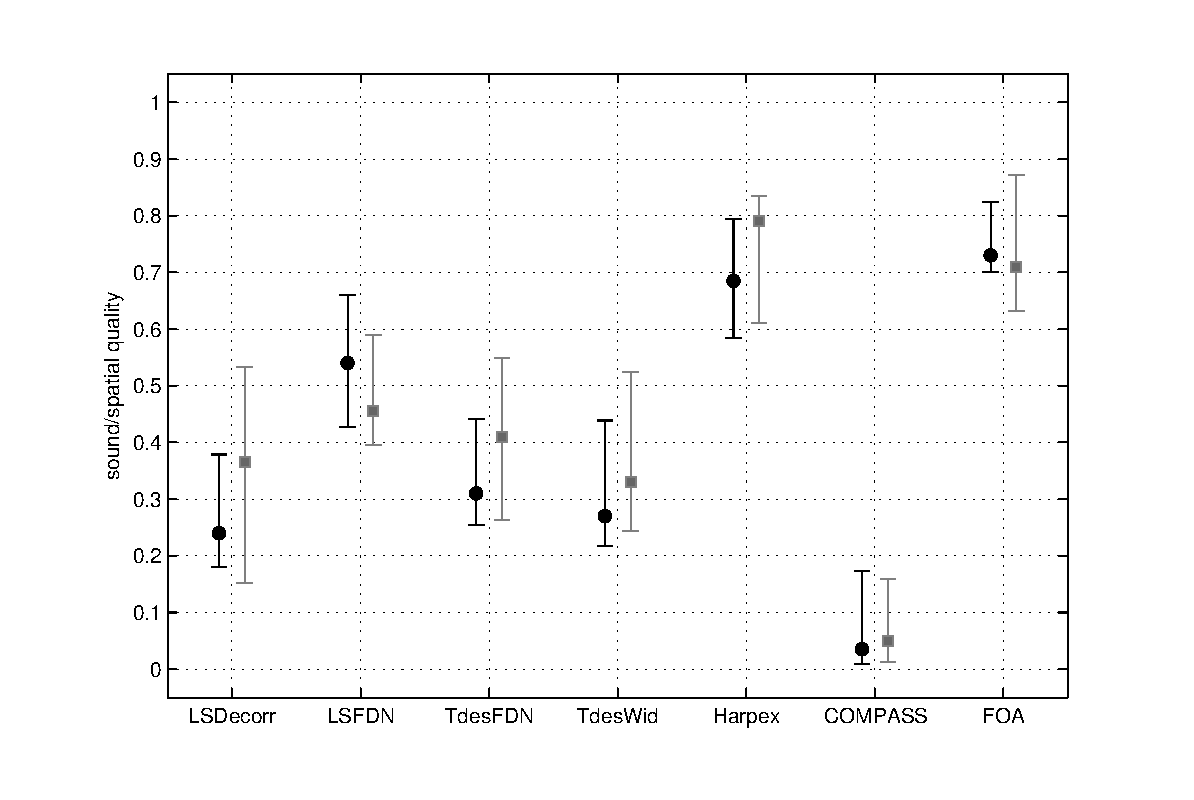
\includegraphics[width=1\textwidth]{ergebnis/plots/result.eps}
  \caption{Ergebnis des Hörversuchs, Median mit 95\% Konfidenzintervalle (Klangqualität in schwarz und räumliche Qualität in grau)}
  \label{fig:versuch}
\end{figure}

Die Bewertungen erfolgten nach zwei Kriterien:

\begin{itemize}
  \item Klangqualität: \textit{sehr gut} (1) bis \textit{sehr schlecht} (0)
  \item räumliche Qualität: \textit{realistisch} (1) bis \textit{synthetisch} (0)
\end{itemize}

Die Bewertungen nach den zwei gewählten Kriterien weisen eine hohe Korrelation auf. Dies deutet entweder auf eine tatsächliche Korrelation der Algorithmen von Klangqualität und räumlicher Wiedergabequalität hin, oder die Fragestellung zielt nicht auf genügend unterschiedliche Aspekte der Testsignale ab. Dabei können stärkere Artefakte als Verminderung der räumlichen Qualität des Algorithmus gedeutet werden.
    \subsection{Diskussion}
    diskussionstext


\section{Fazit}
Die Funktion von DirAC als Upmixingmethode für FOA wurde theoretisch erklärt und in einer Implementierung praktisch angewendet. Es wurden verschiedene Varianten des Algorithmus entwickelt, die sich in den Methoden zur Synthese des Diffusanteils und in der Ambisonics Dekodierung unterschieden. Diese Varianten wurden mit einer Referenz (FOA) und zwei weiteren Upmixingverfahren (HARPEX, COMPASS) in einem Hörversuch verglichen.

Die Bewertungskriterien Klangqualität und räumliche Qualität im Hörversuch wiesen wahrscheinlich auf Grund der Fragestellung bzw. der Benennung der Kriterien einen hohen Zusammanhang in den Bewertungen auf. Die Referenz (FOA) wurde ähnlich gut bewertet wie der am besten bewertetste Upmixingalgorithmus HARPEX, was der Theorie widerspicht. Die Art der Fragestellung im Hörversuch kann auch in diesem Fall eine Erklärung für dieses Resultat sein.

Somit kann mit diesem Hörversuch gezeigt werden, dass nach unseren Kriterien FOA gleichwertig mit HARPEX am besten bewertet wurden und COMPASS am schlechtesten bewertet wurde. Die verschiedenen DirAC Implementierungen liegen dazwischen.

Das Ergebnis des Hörversuchs gibt einen Hinweis darauf, dass eine DirAC Implementierung mit direkter Ambisonics Dekodierung auf die physische Lautsprecheranordnung und einem FDN zur Diffussignnal-Synthese (LSFDN) eine bessere Klangqualität erreichen kann, als die anderen DirAC Varianten in unserem Versuch.


\bibliographystyle{IEEEtranSA}
\bibliography{bib_database}

\newpage
\appendix

\newpage

\section{Anhang: Ergebnisse des Hörversuchs}
% Please add the following required packages to your document preamble:
% \usepackage{graphicx}
\begin{table}[!ht]
\resizebox{\textwidth}{!}{%
\begin{tabular}{|l|l|l|l|l|l|l|l|l|}
\hline
\textbf{Spkr\_Octave\_Decorr} & \textbf{Spkr\_FDN} & \textbf{T-design\_FDN} & \textbf{T-design\_Widening} & \textbf{Harpy} & \textbf{Compass} & \textbf{FOA\_Referenz} & \textbf{scene} & \textbf{participant} \\ \hline
17.0                          & 60.0               & 50.0                   & 10.0                        & 94.0           & 33.0             & 70.0                   & 1              & 1                    \\ \hline
36.0                          & 52.0               & 44.0                   & 41.0                        & 86.0           & 0.0              & 100.0                  & 2              & 1                    \\ \hline
8.0                           & 40.0               & 32.0                   & 25.0                        & 79.0           & 2.0              & 69.0                   & 3              & 1                    \\ \hline
20.0                          & 60.0               & 81.0                   & 60.0                        & 40.0           & 0.0              & 60.0                   & 4              & 1                    \\ \hline
0.0                           & 50.0               & 24.0                   & 12.0                        & 100.0          & 0.0              & 73.0                   & 1              & 2                    \\ \hline
38.0                          & 79.0               & 28.0                   & 21.0                        & 65.0           & 0.0              & 100.0                  & 2              & 2                    \\ \hline
10.0                          & 68.0               & 47.0                   & 25.0                        & 100.0          & 0.0              & 100.0                  & 3              & 2                    \\ \hline
54.0                          & 100.0              & 13.0                   & 23.0                        & 71.0           & 0.0              & 87.0                   & 4              & 2                    \\ \hline
28.0                          & 60.0               & 19.0                   & 25.0                        & 85.0           & 4.0              & 85.0                   & 1              & 3                    \\ \hline
17.0                          & 78.0               & 62.0                   & 19.0                        & 79.0           & 60.0             & 86.0                   & 2              & 3                    \\ \hline
6.0                           & 33.0               & 20.0                   & 77.0                        & 81.0           & 0.0              & 85.0                   & 3              & 3                    \\ \hline
79.0                          & 73.0               & 67.0                   & 40.0                        & 78.0           & 3.0              & 79.0                   & 4              & 3                    \\ \hline
67.0                          & 56.0               & 32.0                   & 50.0                        & 50.0           & 28.0             & 38.0                   & 1              & 4                    \\ \hline
40.0                          & 34.0               & 30.0                   & 16.0                        & 21.0           & 49.0             & 73.0                   & 2              & 4                    \\ \hline
62.0                          & 34.0               & 50.0                   & 44.0                        & 57.0           & 24.0             & 50.0                   & 3              & 4                    \\ \hline
20.0                          & 26.0               & 30.0                   & 56.0                        & 47.0           & 6.0              & 69.0                   & 4              & 4                    \\ \hline
15.0                          & 38.0               & 26.0                   & 49.0                        & 53.0           & 20.0             & 70.0                   & 1              & 5                    \\ \hline
38.0                          & 50.0               & 22.0                   & 15.0                        & 59.0           & 6.0              & 70.0                   & 2              & 5                    \\ \hline
45.0                          & 49.0               & 23.0                   & 29.0                        & 66.0           & 15.0             & 84.0                   & 3              & 5                    \\ \hline
18.0                          & 72.0               & 32.0                   & 50.0                        & 57.0           & 0.0              & 68.0                   & 4              & 5                    \\ \hline
\end{tabular}%
}
\caption {Klangqualität}
\end{table}
% Please add the following required packages to your document preamble:
% \usepackage{graphicx}
\begin{table}[!ht]
\resizebox{\textwidth}{!}{%
\begin{tabular}{|l|l|l|l|l|l|l|l|l|}
\hline
\textbf{Spkr\_Octave\_Decorr} & \textbf{Spkr\_FDN} & \textbf{T-design\_FDN} & \textbf{T-design\_Widening} & \textbf{Harpy} & \textbf{Compass} & \textbf{FOA\_Referenz} & \textbf{scene} & \textbf{participant} \\ \hline
0.0                           & 64.0               & 78.0                   & 0.0                         & 100.0          & 0.0              & 21.0                   & 1              & 1                    \\ \hline
35.0                          & 68.0               & 41.0                   & 0.0                         & 81.0           & 0.0              & 100.0                  & 2              & 1                    \\ \hline
0.0                           & 40.0               & 33.0                   & 22.0                        & 50.0           & 0.0              & 61.0                   & 3              & 1                    \\ \hline
59.0                          & 84.0               & 71.0                   & 26.0                        & 16.0           & 0.0              & 100.0                  & 4              & 1                    \\ \hline
0.0                           & 74.0               & 41.0                   & 62.0                        & 85.0           & 12.0             & 100.0                  & 1              & 2                    \\ \hline
37.0                          & 14.0               & 10.0                   & 22.0                        & 100.0          & 60.0             & 83.0                   & 2              & 2                    \\ \hline
0.0                           & 44.0               & 0.0                    & 62.0                        & 82.0           & 14.0             & 100.0                  & 3              & 2                    \\ \hline
38.0                          & 48.0               & 0.0                    & 11.0                        & 100.0          & 0.0              & 96.0                   & 4              & 2                    \\ \hline
17.0                          & 15.0               & 17.0                   & 58.0                        & 29.0           & 6.0              & 80.0                   & 1              & 3                    \\ \hline
76.0                          & 63.0               & 41.0                   & 14.0                        & 85.0           & 25.0             & 89.0                   & 2              & 3                    \\ \hline
11.0                          & 35.0               & 30.0                   & 62.0                        & 80.0           & 0.0              & 71.0                   & 3              & 3                    \\ \hline
40.0                          & 37.0               & 79.0                   & 37.0                        & 78.0           & 5.0              & 82.0                   & 4              & 3                    \\ \hline
50.0                          & 47.0               & 57.0                   & 81.0                        & 40.0           & 0.0              & 64.0                   & 1              & 4                    \\ \hline
72.0                          & 50.0               & 62.0                   & 36.0                        & 56.0           & 25.0             & 48.0                   & 2              & 4                    \\ \hline
59.0                          & 43.0               & 79.0                   & 40.0                        & 76.0           & 25.0             & 60.0                   & 3              & 4                    \\ \hline
68.0                          & 42.0               & 50.0                   & 21.0                        & 54.0           & 38.0             & 50.0                   & 4              & 4                    \\ \hline
5.0                           & 37.0               & 20.0                   & 30.0                        & 76.0           & 0.0              & 60.0                   & 1              & 5                    \\ \hline
62.0                          & 79.0               & 56.0                   & 27.0                        & 90.0           & 5.0              & 68.0                   & 2              & 5                    \\ \hline
14.0                          & 38.0               & 23.0                   & 48.0                        & 85.0           & 3.0              & 67.0                   & 3              & 5                    \\ \hline
36.0                          & 50.0               & 27.0                   & 60.0                        & 75.0           & 12.0             & 71.0                   & 4              & 5                    \\ \hline
\end{tabular}%
}
\caption {Qualität der räumlichen Darstellung}
\end{table}
Scenes:
\begin{itemize}
    \item 1: Synthetisches Zirpen, rotierend in Azimuth
    \item 2: Synthetisches Zirpen, rotierend in Azimuth, nachträglich verhallt
    \item 3: Live-Musik Aufnahme
    \item 4: Umgebungsgeräusche Straßenkreuzung
\end{itemize}

\end{document}



